\documentclass{beamer}
\usetheme[sectionpage=progressbar, subsectionpage=progressbar, numbering=fraction, progressbar=foot, block=fill, background=light]{metropolis}
\usepackage{appendixnumberbeamer}
\usepackage{textpos}
\usepackage{booktabs}
\usepackage[scale=2]{ccicons}
\usepackage{anyfontsize}
\usepackage{pgfplots}
\usepgfplotslibrary{dateplot}
\usetikzlibrary{backgrounds}
\usepackage{xspace}
\newcommand{\themename}{\textbf{\textsc{metropolis}}\xspace}
\title{Attention based models in End-to-End ASR}
\subtitle{Exploration of Attention in ESPNET toolkit}
\date{\today}
\author{Shreekantha Nadig}
\institute{International Institute of Information Technology - Bangalore}
%\titlegraphic{\hfill\includegraphics[height=1.5cm]{logo.pdf}}

\usepackage{tikz}
\usetikzlibrary{shapes,shadows,arrows,patterns}
\tikzstyle{line} = [draw, -latex']
\tikzstyle{round} = [draw, circle, fill=black!30, minimum size=4em, node distance=4em, font=\fontsize{30}{10}\selectfont]
\tikzstyle{mlp_enc} = [rectangle, draw, fill=red!50, text width=2cm, minimum height=5em, text centered, node distance=10em, font=\fontsize{20}{10}\selectfont]
\tikzstyle{mlp_att} = [rectangle, draw, fill=green!50, text width=2cm, minimum height=5em, text centered, node distance=10em, font=\fontsize{20}{10}\selectfont]
\tikzstyle{mlp_dec} = [rectangle, draw, fill=blue!50, text width=2cm, minimum height=5em, text centered, node distance=10em, font=\fontsize{20}{10}\selectfont]
\tikzstyle{enc_h} = [rectangle, draw,  pattern=horizontal lines, pattern color=red!60, text width=1cm, minimum height=10em, minimum width=3em, text centered, node distance=10em, font=\fontsize{25}{10}\selectfont]
\tikzstyle{atts} = [rectangle, draw,  pattern=horizontal lines, pattern color=green!70, text width=1cm, minimum height=10em, minimum width=3em, text centered, node distance=10em, font=\fontsize{20}{10}\selectfont]
\tikzstyle{dec_z} = [rectangle, draw,  pattern=horizontal lines, pattern color=blue!60, text width=1cm, minimum height=10em, minimum width=3em, text centered, node distance=10em, font=\fontsize{20}{10}\selectfont]
\tikzstyle{cnn} = [rectangle, draw,  pattern=crosshatch, pattern color=red!50!blue!50, text width=2cm, minimum height=5em, text centered, node distance=10em, font=\fontsize{20}{10}\selectfont]
\tikzstyle{box} = [rectangle, draw,  fill=blue!20, text width=3cm, minimum height=5em, minimum width=3em, text centered, node distance=10em, font=\fontsize{20}{10}\selectfont]

\begin{document}
\addtobeamertemplate{frametitle}{}{%
	\begin{textblock*}{100mm}(.97\textwidth,-1cm)
		{
\includegraphics[width=2.5em]{iiitb_logo.png}}
	\end{textblock*}}
\maketitle

\begin{frame}{Table of contents}
	\setbeamertemplate{section in toc}[sections numbered]
	\tableofcontents[hideallsubsections]
\end{frame}

\section{AttDot}
\section{Introduction}
	\begin{frame}[fragile]{Additive Attention}
	\begin{center}
		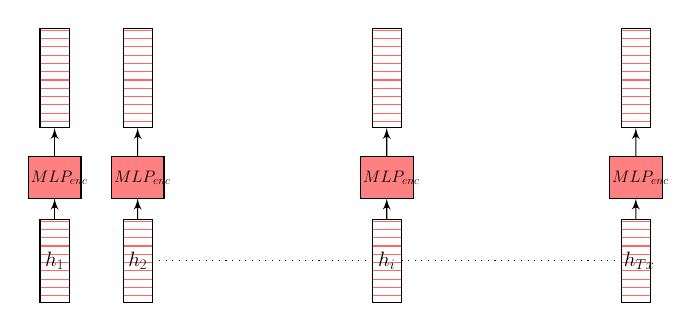
\begin{tikzpicture}[scale=0.3, every node/.style={transform shape}]
		\node [enc_h] (h1) {$h_{1}$};
		\node [enc_h,right of = h1] (h2) {$h_{2}$};
		\node [enc_h,right of = h2, node distance = 30em] (hi) {$h_{i}$};
		\node [enc_h,right of = hi, node distance = 30em] (hTx) {$h_{Tx}$};
		\draw [dotted] (h2.east) to (hi.west);
		\draw [dotted] (hi.east) to (hTx.west);
		\pause{}
		
		\node [mlp_enc, above of = h1, node distance = 10em] (mlp1) {$MLP_{enc}$};
		\path [line] (h1.north) to (mlp1.south);
		\node [enc_h, above of = mlp1, minimum height = 12em, node distance = 12em] (he1) {};
		\path [line] (mlp1.north) to (he1.south);
		
		\pause{}
		\node [mlp_enc, above of = h2, node distance = 10em] (mlp2) {$MLP_{enc}$};
		\path [line] (h2.north) to (mlp2.south);
		\node [enc_h, above of = mlp2, minimum height = 12em, node distance = 12em] (he2) {};
		\path [line] (mlp2.north) to (he2.south);
		
		\pause{}
		\node [mlp_enc, above of = hi, node distance = 10em] (mlpi) {$MLP_{enc}$};
		\path [line] (hi.north) to (mlpi.south);
		\node [enc_h, above of = mlpi, minimum height = 12em, node distance = 12em] (hei) {};
		\path [line] (mlpi.north) to (hei.south);
		
		\pause{}
		\node [mlp_enc, above of = hTx, node distance = 10em] (mlpTx) {$MLP_{enc}$};
		\path [line] (hTx.north) to (mlpTx.south);
		\node [enc_h, above of = mlpTx, minimum height = 12em, node distance = 12em] (heTx) {};
		\path [line] (mlpTx.north) to (heTx.south);
		\end{tikzpicture}
	\end{center}
	\end{frame}

	\begin{frame}[fragile]{Additive Attention}
	\begin{center}
		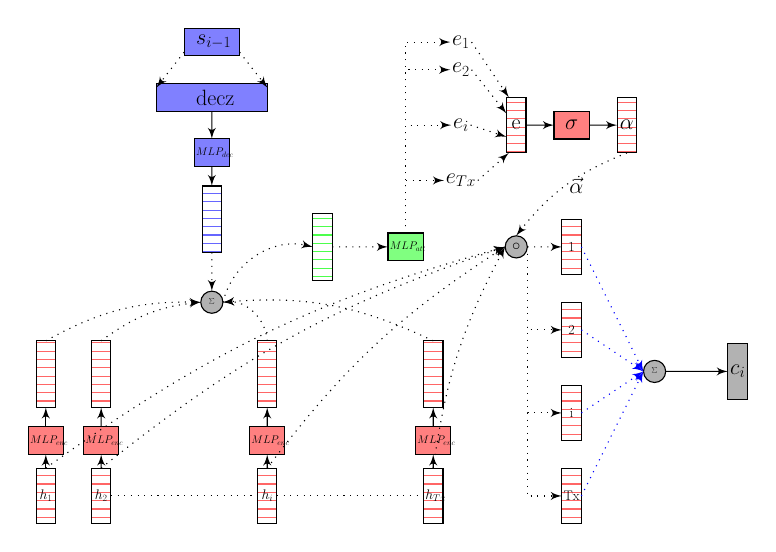
\begin{tikzpicture}[scale=0.2, every node/.style={transform shape}]
		\node [enc_h] (h1) {$h_{1}$};
		\node [enc_h,right of = h1] (h2) {$h_{2}$};
		\node [enc_h,right of = h2, node distance = 30em] (hi) {$h_{i}$};
		\node [enc_h,right of = hi, node distance = 30em] (hTx) {$h_{Tx}$};
		\draw [dotted] (h2.east) to (hi.west);
		\draw [dotted] (hi.east) to (hTx.west);
		
		
		\node [mlp_enc, above of = h1, node distance = 10em] (mlp1) {$MLP_{enc}$};
		\path [line] (h1.north) to (mlp1.south);
		\node [enc_h, above of = mlp1, minimum height = 12em, node distance = 12em] (he1) {};
		\path [line] (mlp1.north) to (he1.south);
		
		
		\node [mlp_enc, above of = h2, node distance = 10em] (mlp2) {$MLP_{enc}$};
		\path [line] (h2.north) to (mlp2.south);
		\node [enc_h, above of = mlp2, minimum height = 12em, node distance = 12em] (he2) {};
		\path [line] (mlp2.north) to (he2.south);
		
		
		\node [mlp_enc, above of = hi, node distance = 10em] (mlpi) {$MLP_{enc}$};
		\path [line] (hi.north) to (mlpi.south);
		\node [enc_h, above of = mlpi, minimum height = 12em, node distance = 12em] (hei) {};
		\path [line] (mlpi.north) to (hei.south);
		
		
		\node [mlp_enc, above of = hTx, node distance = 10em] (mlpTx) {$MLP_{enc}$};
		\path [line] (hTx.north) to (mlpTx.south);
		\node [enc_h, above of = mlpTx, minimum height = 12em, node distance = 12em] (heTx) {};
		\path [line] (mlpTx.north) to (heTx.south);
		
		\node [mlp_dec, above of = hei, node distance = 60em, minimum width = 10em, xshift = -10em, font=\fontsize{40}{10}\selectfont] (sim1) {$s_{i-1}$};
		\node [mlp_dec, below of=sim1, minimum width = 20em, font=\fontsize{40}{10}\selectfont] (dec_z) {decz};
		\path [line, dotted] (sim1.200) to (dec_z.170);
		\path [line, dotted] (sim1.-20) to (dec_z.10);
		\node [mlp_dec, below of=dec_z, node distance = 10em] (mlp_dec) {$MLP_{dec}$};
		\path [line] (dec_z) to (mlp_dec);
		\node [dec_z, below of = mlp_dec, minimum height = 12em, node distance = 12em] (decz_enc) {};
		\path [line] (mlp_dec) to (decz_enc);

		\uncover<2-7>{
		\node [round, below of = decz_enc, node distance = 15em] (prod) {$\sum$}; 
		\path [line, dotted] (decz_enc.south) to (prod.north);
		\uncover<2-4>{
		\path [line, dotted] (he1.north) to [bend left=15] (prod.west);
		}
		\node [atts, right of = prod, minimum height = 12em, node distance = 20em, yshift=10em] (h_z) {};
		\path [line, dotted] (prod.east) to [bend left=45] (h_z.west);
		}

		\uncover<3-7>{
		\node [mlp_att, right of = h_z, node distance = 15em] (sum) {$MLP_{att}$};
%		\node [round, right of = h_z, node distance = 15em] (sum) {$\sum$};
		\path [line, dotted] (h_z.east) to (sum.west);
		}
	
		\uncover<4->{
		\node [right of=sim1, node distance = 15em, xshift=30em, font=\fontsize{40}{10}\selectfont] (e1) {$e_{1}$};
		\uncover<4>{
		\path [line, dotted] (sum.north) |- (e1.west);
		}
		}
	
		\uncover<5->{
		\node [below of=e1, node distance = 5em, font=\fontsize{40}{10}\selectfont] (e2) {$e_{2}$};
		\uncover<5>{
		\path [line, dotted] (he2.north) to [bend left=15] (prod.west);
		\path [line, dotted] (sum.north) |- (e2.west);
		}
		}
	
		\uncover<6->{
		\node [below of=e2, node distance = 10em, font=\fontsize{40}{10}\selectfont] (ei) {$e_{i}$};
		\uncover<6>{
		\path [line, dotted] (hei.north) to [bend right=45] (prod.east);
		\path [line, dotted] (sum.north) |- (ei.west);
		}
		}
		
		\uncover<7->{
		\node [below of=ei, node distance = 10em, font=\fontsize{40}{10}\selectfont] (eTx) {$e_{Tx}$};
		\only<7>{
		\path [line, dotted] (heTx.north) to [bend right=15] (prod.east);
		\path [line, dotted] (sum.north) |- (eTx.west);
		}
		}

		\uncover<8->{
		\node [enc_h, right of=ei, font=\fontsize{40}{10}\selectfont] (e) {e};
		

		\path [line, dotted] (e1.east) to (e.105);
		\path [line, dotted] (e2.east) to (e.130);
		\path [line, dotted] (ei.east) to (e.-130);
		\path [line, dotted] (eTx.east) to (e.-105);
		

		\node [mlp_enc, right of=e, font=\fontsize{40}{10}\selectfont] (sm) {$\sigma$};
		\path [line] (e.east) to (sm.west);
		

		\node [enc_h, right of=sm, font=\fontsize{40}{10}\selectfont] (alphas) {$\alpha$};
		\path [line] (sm.east) to (alphas.west);
		}
		\uncover<9>{
		\node [round, right of=sum, node distance=20em] (alpha_h) {$\circ$};
		\path [line, dotted, color=black] (h1.north) to [bend left=10] (alpha_h.west);
		\path [line, dotted, color=black] (alphas.south) to [bend right=15] node [xshift=2em] {\fontsize{40}{10}\selectfont $\vec{\alpha}$} (alpha_h.north);
		

		\node [enc_h, right of=alpha_h] (ahe1) {1};
		\path [line, dotted, color=black] (alpha_h.east) to (ahe1.west);
		
		\path [line, dotted, color=black] (h2.north) to [bend left=10] (alpha_h.west);
		\node [enc_h, below of=ahe1, node distance = 15em] (ahe2) {2};
		\path [line, dotted, color=black] (alpha_h.east) |- (ahe2.west);
		

		\path [line, dotted, color=black] (hi.north) to [bend left=10] (alpha_h.west);
		\node [enc_h, below of=ahe2, node distance = 15em] (ahei) {i};
		\path [line, dotted, color=black] (alpha_h.east) |- (ahei.west);
		
		\path [line, dotted, color=black] (hTx.north) to [bend left=10] (alpha_h.west);
		\node [enc_h, below of=ahei, node distance = 15em] (aheTx) {Tx};
		\path [line, dotted, color=black] (alpha_h.east) |- (aheTx.west);
		
		\pause{}
		\node [round, right of=ahe2, yshift=-7.5em, node distance = 15em] (sum_op) {$\sum$};
		\path [line, dotted, color=blue] (ahe1.east) to (sum_op.west);
		\path [line, dotted, color=blue] (ahe2.east) to (sum_op.west);
		\path [line, dotted, color=blue] (ahei.east) to (sum_op.west);
		\path [line, dotted, color=blue] (aheTx.east) to (sum_op.west);
		
		\pause{}
		\node [enc_h, right of=sum_op, fill=black!30, node distance=15em, font=\fontsize{40}{10}\selectfont] (ci) {$c_i$};
		\path [line] (sum_op.east) to (ci.west);
		}
		\end{tikzpicture}
	\end{center}
	\end{frame}


	\begin{frame}[fragile]{Additive Attention - Full picture}
	\begin{center}
		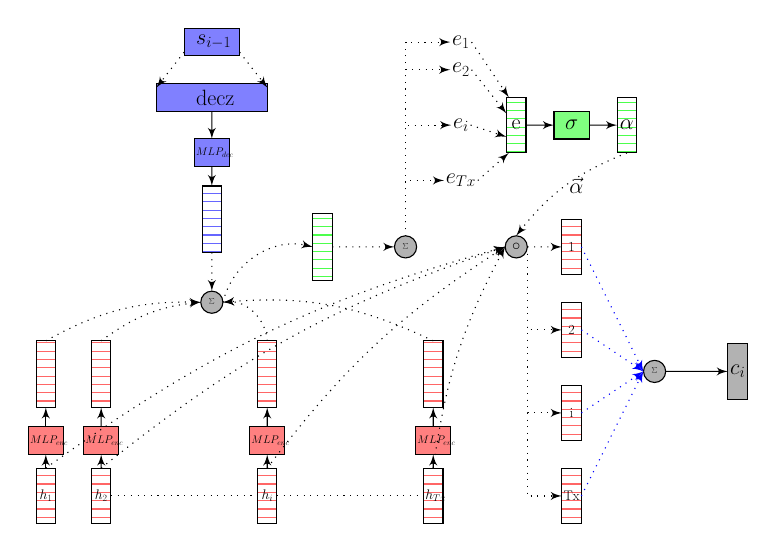
\begin{tikzpicture}[scale=0.2, every node/.style={transform shape}]
		\node [enc_h] (h1) {$h_{1}$};
		\node [enc_h,right of = h1] (h2) {$h_{2}$};
		\node [enc_h,right of = h2, node distance = 30em] (hi) {$h_{i}$};
		\node [enc_h,right of = hi, node distance = 30em] (hTx) {$h_{Tx}$};
		\draw [dotted] (h2.east) to (hi.west);
		\draw [dotted] (hi.east) to (hTx.west);
		
		
		\node [mlp_enc, above of = h1, node distance = 10em] (mlp1) {$MLP_{enc}$};
		\path [line] (h1.north) to (mlp1.south);
		\node [enc_h, above of = mlp1, minimum height = 12em, node distance = 12em] (he1) {};
		\path [line] (mlp1.north) to (he1.south);
		
		
		\node [mlp_enc, above of = h2, node distance = 10em] (mlp2) {$MLP_{enc}$};
		\path [line] (h2.north) to (mlp2.south);
		\node [enc_h, above of = mlp2, minimum height = 12em, node distance = 12em] (he2) {};
		\path [line] (mlp2.north) to (he2.south);
		
		
		\node [mlp_enc, above of = hi, node distance = 10em] (mlpi) {$MLP_{enc}$};
		\path [line] (hi.north) to (mlpi.south);
		\node [enc_h, above of = mlpi, minimum height = 12em, node distance = 12em] (hei) {};
		\path [line] (mlpi.north) to (hei.south);
		
		
		\node [mlp_enc, above of = hTx, node distance = 10em] (mlpTx) {$MLP_{enc}$};
		\path [line] (hTx.north) to (mlpTx.south);
		\node [enc_h, above of = mlpTx, minimum height = 12em, node distance = 12em] (heTx) {};
		\path [line] (mlpTx.north) to (heTx.south);
		
		\node [mlp_dec, above of = hei, node distance = 60em, minimum width = 10em, xshift = -10em, font=\fontsize{40}{10}\selectfont] (sim1) {$s_{i-1}$};
		\node [mlp_dec, below of=sim1, minimum width = 20em, font=\fontsize{40}{10}\selectfont] (dec_z) {decz};
		\path [line, dotted] (sim1.200) to (dec_z.170);
		\path [line, dotted] (sim1.-20) to (dec_z.10);
		\node [mlp_dec, below of=dec_z, node distance = 10em] (mlp_dec) {$MLP_{dec}$};
		\path [line] (dec_z) to (mlp_dec);
		\node [dec_z, below of = mlp_dec, minimum height = 12em, node distance = 12em] (decz_enc) {};
		\path [line] (mlp_dec) to (decz_enc);
		
	
		\node [round, below of = decz_enc, node distance = 15em] (prod) {$\sum$}; 
		\path [line, dotted] (decz_enc.south) to (prod.north);
	
		\path [line, dotted] (he1.north) to [bend left=15] (prod.west);
		\node [atts, right of = prod, minimum height = 12em, node distance = 20em, yshift=10em] (h_z) {};
		\path [line, dotted] (prod.east) to [bend left=45] (h_z.west);
		
	
			\node [round, right of = h_z, node distance = 15em] (sum) {$\sum$};
			\path [line, dotted] (h_z.east) to (sum.west);
			
			
			
			\node [right of=sim1, node distance = 15em, xshift=30em, font=\fontsize{40}{10}\selectfont] (e1) {$e_{1}$};
			
			\path [line, dotted] (sum.north) |- (e1.west);
			
			\node [below of=e1, node distance = 5em, font=\fontsize{40}{10}\selectfont] (e2) {$e_{2}$};
			
			\path [line, dotted] (he2.north) to [bend left=15] (prod.west);
			\path [line, dotted] (sum.north) |- (e2.west);
			
			
			
			\node [below of=e2, node distance = 10em, font=\fontsize{40}{10}\selectfont] (ei) {$e_{i}$};
			
			\path [line, dotted] (hei.north) to [bend right=45] (prod.east);
			\path [line, dotted] (sum.north) |- (ei.west);
			
			
			
			\node [below of=ei, node distance = 10em, font=\fontsize{40}{10}\selectfont] (eTx) {$e_{Tx}$};
			
			\path [line, dotted] (heTx.north) to [bend right=15] (prod.east);
			\path [line, dotted] (sum.north) |- (eTx.west);
			
			
			\node [atts, right of=ei, font=\fontsize{40}{10}\selectfont] (e) {e};
			
			
			\path [line, dotted] (e1.east) to (e.105);
			\path [line, dotted] (e2.east) to (e.130);
			\path [line, dotted] (ei.east) to (e.-130);
			\path [line, dotted] (eTx.east) to (e.-105);
			
			
			\node [mlp_att, right of=e, font=\fontsize{40}{10}\selectfont] (sm) {$\sigma$};
			\path [line] (e.east) to (sm.west);
			
			
			\node [atts, right of=sm, font=\fontsize{40}{10}\selectfont] (alphas) {$\alpha$};
			\path [line] (sm.east) to (alphas.west);
			
			
			\node [round, right of=sum, node distance=20em] (alpha_h) {$\circ$};
			\path [line, dotted, color=black] (h1.north) to [bend left=10] (alpha_h.west);
			\path [line, dotted, color=black] (alphas.south) to [bend right=15] node [xshift=2em] {\fontsize{40}{10}\selectfont $\vec{\alpha}$} (alpha_h.north);
			
			
			\node [enc_h, right of=alpha_h] (ahe1) {1};
			\path [line, dotted, color=black] (alpha_h.east) to (ahe1.west);
			
			\path [line, dotted, color=black] (h2.north) to [bend left=10] (alpha_h.west);
			\node [enc_h, below of=ahe1, node distance = 15em] (ahe2) {2};
			\path [line, dotted, color=black] (alpha_h.east) |- (ahe2.west);
			
			
			\path [line, dotted, color=black] (hi.north) to [bend left=10] (alpha_h.west);
			\node [enc_h, below of=ahe2, node distance = 15em] (ahei) {i};
			\path [line, dotted, color=black] (alpha_h.east) |- (ahei.west);
			
			\path [line, dotted, color=black] (hTx.north) to [bend left=10] (alpha_h.west);
			\node [enc_h, below of=ahei, node distance = 15em] (aheTx) {Tx};
			\path [line, dotted, color=black] (alpha_h.east) |- (aheTx.west);
			
			\node [round, right of=ahe2, yshift=-7.5em, node distance = 15em] (sum_op) {$\sum$};
			\path [line, dotted, color=blue] (ahe1.east) to (sum_op.west);
			\path [line, dotted, color=blue] (ahe2.east) to (sum_op.west);
			\path [line, dotted, color=blue] (ahei.east) to (sum_op.west);
			\path [line, dotted, color=blue] (aheTx.east) to (sum_op.west);
			
			
			\node [enc_h, right of=sum_op, fill=black!30, node distance=15em, font=\fontsize{40}{10}\selectfont] (ci) {$c_i$};
			\path [line] (sum_op.east) to (ci.west);
		\end{tikzpicture}
	\end{center}
	\end{frame}
\end{document}
